\documentclass{beamer}
\usetheme{Madrid}
% \usecolortheme{beaver} 
% \setbeamercolor{palette primary}{bg=orange, fg=white}
\title{Analysis of the SlateQ Algorithm}
\author{Your Name}
\date{\today}

\usepackage{amsmath} % for align environment

\begin{document}

% Slide 1: Introduction to SlateQ
\begin{frame}{SlateQ vs. Tabular Q-Learning}
\begin{itemize}
    \item In tabular Q-Learning:
    \begin{equation*}
    Q^t(s,A) = Q^{t-1}(s,A) + \alpha\left(R(s,A,s') + \max_{A'}\left(\gamma Q^{t-1}(s',A')\right) - Q^{t-1}(s,A)\right)
    \end{equation*}
    \item Dimension of $Q(s,A)$: $K\times {K \choose N}$. Time-consuming for large $K$ and $N$.
    \item SlateQ introduces $\bar{Q}(s,i)$ to avoid exhaustive exploration. 
    \item Updated using:
    \begin{align*}
        \bar{Q}^t(s,i) &= \bar{Q}^{t-1}(s,i) \\
        &\quad + \alpha\left(R(s,A,s') + \max_{A'}\left(\gamma Q^{t-1}(s',A')\right) - \bar{Q}^{t-1}(s,i)\right)
    \end{align*}
\end{itemize}
\end{frame}

% Slide 2: Maximization Problem
\begin{frame}{Maximization Problem in SlateQ}
\begin{itemize}
    \item In our environment:
    \begin{equation*}
    Q(s,A) = \sum_{i\in A}P(i|s,A)\bar{Q}(s,i)
    \end{equation*}
    \item Revised update equation:
    \begin{align*}
        \bar{Q}^t(s,i) &= \bar{Q}^{t-1}(s,i) \\
        &\quad + \alpha\left(R(s,i) + \max_{A'}\left(\gamma \sum_{j\in A'}P^{t-1}(j|i,A')\bar{Q}^{t-1}(i,j)\right) - \bar{Q}^{t-1}(s,i)\right)
    \end{align*}
    \item Maximization problem:
    \begin{align*}
    \max_{A}\sum_{i\in A}P(i|s,A)\bar{Q}(s,i) &= \max_{A}\sum_{i\in A}\frac{1}{N}\bar{Q}(s,i) 
    \end{align*}
    Linear optimization:
    \begin{align*}
    \max_{\bf x} \sum_i x_i\frac{1}{N}\bar{Q}(s,i) \quad \text{s.t.} \quad &x_i \in [0,1], \\
    &\sum_{i} x_i = N
    \end{align*}
\end{itemize}
\end{frame}

% Slide 1: Evaluation Description and Optimal Average Cost
\begin{frame}{Evaluation Description and Optimal Average Cost}
    \begin{itemize}
        \item Evaluate algorithm's effectiveness using a simulation function.
        \item Calculate average cost per session using the derived policy.
        \item For fixed number of cached items $C=0.2K$, the optimal average cost, $E(S)$, is:
        \begin{equation*}
            E[S] = 0.8 + 0.8(\frac{1}{q}-1)(1-\alpha)
        \end{equation*}
        \item With $\alpha = 0.8$ and $q=0.2$, we get $E[S] = 1.44$.
        \item Optimal policy should yield this average cost.
    \end{itemize}
    \end{frame}
    
    % Slide 2: Simulation Results and Analysis
    \begin{frame}{Simulation Results and Analysis}
    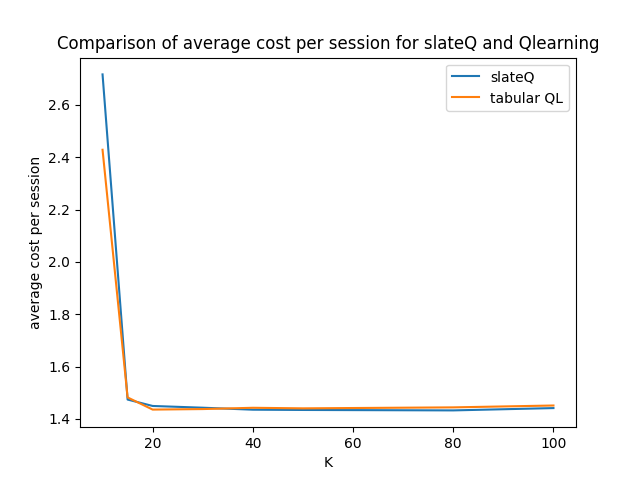
\includegraphics[width=0.48\linewidth]{Figure_1.png}
    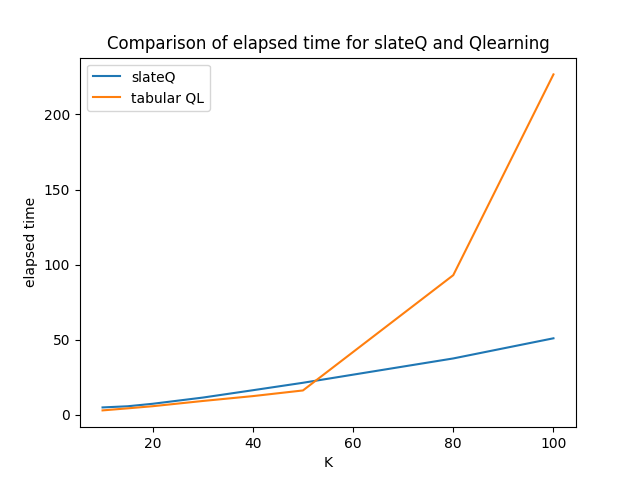
\includegraphics[width=0.48\linewidth]{Figure_2.png}
    \begin{itemize}
        \item Average cost for SlateQ aligns with Q-Learning and converges to $1.44$.
        \item SlateQ time increases linearly with $K$, Q-Learning escalates exponentially.
    \end{itemize}
\end{frame}
    \begin{frame}{Simulation Results and Analysis}
    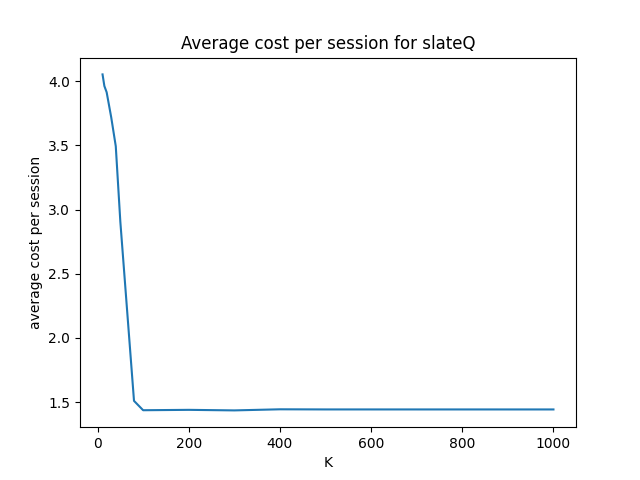
\includegraphics[width=0.48\linewidth]{Figure_3.png}
    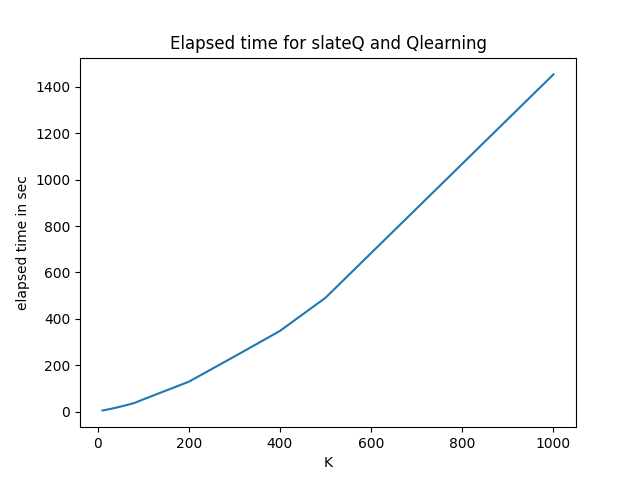
\includegraphics[width=0.48\linewidth]{Figure_4.png}
    \begin{itemize}
        \item With a large library, the algorithm identifies optimal policy, cost remains $1.44$.
        \item Elapsed time exhibits a near-linear increase. Algorithm operates as expected.
    \end{itemize}
    \end{frame}

\end{document}
